% -*- Mode:TeX -*-

%% The documentclass options along with the pagestyle can be used to generate
%% a technical report, a draft copy, or a regular thesis.  You may need to
%% re-specify the pagestyle after you \include  cover.tex.  For more
%% information, see the first few lines of mitthesis.cls.

%\documentclass[12pt,vi,twoside]{mitthesis}
%%
%%  If you want your thesis copyright to you instead of MIT, use the
%%  ``vi'' option, as above.
%%
%\documentclass[12pt,twoside,leftblank]{mitthesis}
%%
%% If you want blank pages before new chapters to be labelled ``This
%% Page Intentionally Left Blank'', use the ``leftblank'' option, as
%% above.

\documentclass[12pt,vi,twoside]{mitthesis}
\usepackage{lgrind}
\pagestyle{plain}

%\usepackage{graphicx,epsfig,amsfonts,amssymb,amsmath,subfigure,setspace,url,wrapfig,caption,boxedminipage,multirow}
\usepackage{graphicx,epsfig,amsfonts,amssymb,amsmath,url,caption}

%% This bit allows you to either specify only the files which you wish to
%% process, or `all' to process all files which you \include.
%% Krishna Sethuraman (1990).

%\typein [\files]{Enter file names to process, (chap1,chap2 ...), or `all' to
%process all files:}
%\def\all{all}
%\ifx\files\all \typeout{Including all files.} \else \typeout{Including only \files.} \includeonly{\files} \fi

%\includeonly{chapter5/chapter5}
%\includeonly{appa/appa}

\setlength{\marginparwidth}{1in}
\raggedbottom

% EXTRA CODE: remove this section in final copy
%\usepackage{ifpdf,showkeys}
% \usepackage{xcolor}
%\newcommand{\jsec}[1]{\marginpar{\fcolorbox{yellow}{yellow}{\parbox{0.7in}{\raggedright \color{blue} \tiny #1 }}}}
%\newcommand{\hsec}[1]{\vfill \fcolorbox{lime}{lime}{\parbox{5in}{\raggedright \bf \color{black} #1 }}}
%  
\newif\ifPDF
\ifx\pdfoutput\undefined\PDFfalse \else\ifnum\pdfoutput > 0\PDFtrue
\else\PDFfalse \fi \fi
%  
 \ifPDF \usepackage{float}
%   \usepackage[pdftex, pdfstartview={FitH}, pdfpagelayout={TwoColumnLeft},bookmarksopen=false, plainpages = false, colorlinks=true, citecolor = blue, urlcolor = blue, filecolor=blue , pagecolor=red, pagebackref=true, linkcolor=blue, hypertexnames=false, plainpages=false, pdfpagelabels ]{hyperref}

\usepackage[pdftex, pdfstartview={FitH}, pdfpagelayout={TwoColumnLeft},bookmarksopen=false, plainpages = false, colorlinks=false, pagebackref=true, hypertexnames=false, plainpages=false, pdfpagelabels ]{hyperref}
 \fi
% end of EXTRA CODE

\usepackage[numbers,sort&compress]{natbib}

\usepackage{listings}
\usepackage{placeins}

 
% "define" Scala
\lstdefinelanguage{scala}{
  morekeywords={abstract,case,catch,class,def,%
    do,else,extends,false,final,finally,%
    for,if,implicit,import,match,mixin,%
    new,null,object,override,package,%
    private,protected,requires,return,sealed,%
    super,this,throw,trait,true,try,%
    type,val,var,while,with,yield},
  otherkeywords={=>,<-,<\%,<:,>:,\#,@},
  sensitive=true,
  morecomment=[l]{//},
  morecomment=[n]{/*}{*/},
  morestring=[b]",
  morestring=[b]',
  morestring=[b]"""
}


% PS: extra macros, definitions, etc.
%\usepackage{algorithm}
%\usepackage{algorithmicx}
%\usepackage{algpseudocode}
%\usepackage{multirow}

\newcommand{\insane}{\textsf{Insane}}


\begin{document}

% -*-latex-*-
% $Log: cover.tex,v $
% Revision 1.7  2001/02/08 18:53:16  boojum
% changed some \newpages to \cleardoublepages
%
% Revision 1.6  1999/10/21 14:49:31  boojum
% changed comment referring to documentstyle
%
% Revision 1.5  1999/10/21 14:39:04  boojum
% *** empty log message ***
%
% Revision 1.4  1997/04/18  17:54:10  othomas
% added page numbers on abstract and cover, and made 1 abstract
% page the default rather than 2.  (anne hunter tells me this
% is the new institute standard.)
%
% Revision 1.4  1997/04/18  17:54:10  othomas
% added page numbers on abstract and cover, and made 1 abstract
% page the default rather than 2.  (anne hunter tells me this
% is the new institute standard.)
%
% Revision 1.3  93/05/17  17:06:29  starflt
% Added acknowledgments section (suggested by tompalka)
%
% Revision 1.2  92/04/22  13:13:13  epeisach
% Fixes for 1991 course 6 requirements
% Phrase "and to grant others the right to do so" has been added to
% permission clause
% Second copy of abstract is not counted as separate pages so numbering works
% out
%
% Revision 1.1  92/04/22  13:08:20  epeisach
\title{Toward Interprocedural Effect and Pointer Analysis for Scala}

\author{Etienne Kneuss}

\prevdegrees{
BSc., Computer Science\\
\'{E}cole Polytechnique F\'{e}d\'{e}rale de Lausanne (2009) }

\department{School of Computer and Communication Sciences}
% If the thesis is for two degrees simultaneously, list them both
% separated by \and like this:
% \degree{Doctor of Philosophy \and Master of Science}
\degree{Master of Science in Computer Science}
\degreemonth{August}
\degreeyear{2011}
\thesisdate{June 24, 2011}

%% By default, the thesis will be copyrighted to MIT.  If you need to copyright
%% the thesis to yourself, just specify the `vi' documentclass option.  If for
%% some reason you want to exactly specify the copyright notice text, you can
%% use the \copyrightnoticetext command.
%\copyrightnoticetext{\copyright IBM, 1990.  Do not open till Xmas.}

% If there is more than one supervisor, use the \supervisor command
% once for each.
\supervisor{Viktor Kuncak}{Assistant Professor}
\supervisor{Philippe Suter}{Ph.D. Student}

% This is the department committee chairman, not the thesis committee
% chairman.  You should replace this with your Department's Committee
% Chairman.
\chairman{Prof. XXX}{Associate Department Head\\Chair,
Committee on Graduate Students}

% Make the titlepage based on the above information.  If you need
% something special and can't use the standard form, you can specify
% the exact text of the titlepage yourself.  Put it in a titlepage
% environment and leave blank lines where you want vertical space.
% The spaces will be adjusted to fill the entire page.  The dotted
% lines for the signatures are made with the \signature command.
\maketitle

% The abstractpage environment sets up everything on the page except
% the text itself.  The title and other header material are put at the
% top of the page, and the supervisors are listed at the bottom.  A
% new page is begun both before and after.  Of course, an abstract may
% be more than one page itself.  If you need more control over the
% format of the page, you can use the abstract environment, which puts
% the word "Abstract" at the beginning and single spaces its text.

%% You can either \input (*not* \include) your abstract file, or you can put
%% the text of the abstract directly between the \begin{abstractpage} and
%% \end{abstractpage} commands.

% First copy: start a new page, and save the page number.
\cleardoublepage
% Uncomment the next line if you do NOT want a page number on your
% abstract and acknowledgments pages.
% \pagestyle{empty}
\setcounter{savepage}{\thepage}
\begin{abstractpage}
Static program analysis techniques working on object-oriented languages usually
require precise knowledge of the aliasing relation between variables. This
knowledge is, amongs other things, important to understand the actual effects
of method calls on objects. We developed an analysis combining a pointer analysis
coupled with a memory-based effects analysis for the Scala programming
language. This analysis is based on abstract interpretation, and represents the
effects of methods in a graph representation. This representation allows the
analysis to be compositional. We also provide the implementation of this
analysis in \insane, a freely-available extension of the Scala compiler.

\end{abstractpage}

% Additional copy: start a new page, and reset the page number.  This way,
% the second copy of the abstract is not counted as separate pages.
% Uncomment the next 6 lines if you need two copies of the abstract
% page.
% \setcounter{page}{\thesavepage}
% \begin{abstractpage}
% Static program analysis techniques working on object-oriented languages usually
require precise knowledge of the aliasing relation between variables. This
knowledge is, amongs other things, important to understand the actual effects
of method calls on objects. We developed an analysis combining a pointer analysis
coupled with a memory-based effects analysis for the Scala programming
language. This analysis is based on abstract interpretation, and represents the
effects of methods in a graph representation. This representation allows the
analysis to be compositional. We also provide the implementation of this
analysis in \insane, a freely-available extension of the Scala compiler.

% \end{abstractpage}

\cleardoublepage

\section*{Acknowledgments}
First and foremost I would like to thank my supervisor, Viktor Kuncak, for his
sustained enthousiasm, inspired suggestions and exemplary guidance thourough
the course of this thesis. I would also like to thank him for giving me the
opportunity to work on such interesting subjects, and look forward to working
with him as I continue with my research. I would also like to thank Philippe
Suter for his continuous feedback and guidance without which this thesis would
not have been possible.

I would like to extend my sincere thanks to the members of the Laboratory for
Automated Research and Reasonning for numerous stimulating discussions: Ali,
Andrej, Eva, Giuliano, Hossein, Ruzica, Swen and Tihomir: thanks. I would also
like to thank Lukas Rytz for his patience and technical support regarding the
Scala compiler. Finally I thank those who continuously supported me; my
family, my friends, and of course Aline.




%%%%%%%%%%%%%%%%%%%%%%%%%%%%%%%%%%%%%%%%%%%%%%%%%%%%%%%%%%%%%%%%%%%%%%
% -*-latex-*-

\pagestyle{plain}
  % -*- Mode:TeX -*-
%% This file simply contains the commands that actually generate the table of
%% contents and lists of figures and tables.  You can omit any or all of
%% these files by simply taking out the appropriate command.  For more
%% information on these files, see appendix C.3.3 of the LaTeX manual. 
\tableofcontents
%\newpage
%\listoffigures
%\newpage
%\listoftables


\chapter{Introduction} \label{chap:intro}
%Pointer analysis is a static analysis technique that builds information on the
%relations between pointers and allocated objects. It is also often refered to
%as points-to or alias analysis.
%
%In most object oriented languages such as Scala, the use of pointers is
%overwhelming, rendering even basic static analyses techniques brittle. It is
%thus ofen necessary to establish information on the aliasing relations between
%variables, as well as some knowledge of the shape of structures stored in the
%heap.

\section{Organization of this thesis}
The rest of this thesis is organized as follows: Chapter~\ref{chap:previous}
describes previous work done in the field of pointer analysis.  Then,
Chapter~\ref{chap:overview} gives a quick overview of the tool, followed by
in-depth description of the initial analysis phases.
Chapter~\ref{chap:pointer} describes in full details the pointer analysis
phase.  In Chapter~\ref{chap:implementation}, we describe some technical
implementation details. We then conclude in Chapter~\ref{chap:conclusion} with
some ideas for future work.

\chapter{Tool Overview}
\label{chap:overview}
The tool is made of five distinct phases that are topologically ordered in terms
of requirements. We briefly describe each of the phases necessary for the
overall analysis. Every major phases is later described in full details in
their respective section.
The tool is decomposed as follows, in order:
\begin{enumerate}
    \item{Function Extraction}: extracts function definitions seen in the code, as well as
    assertions or requirements.

    \item{CFG Generation}: generates a control flow graph for each function
    definition, composed of simple assign statements.

    \item{Class Hierarchy}: collects information in order to find all subclasses of a class.

    \item{Type Analysis}: analyzes potential runtime types and builds initial callgraph.

    \item{Pointer Analysis}: analyzes aliasing effects occurring in each
    function. This phase is described in full-details in
    Chapter~\ref{chap:pointer}.
\end{enumerate}

\section{Function Extraction}
Each function definition seen in the code is first collected. We start by
extracting invariants as well as pre- and post- conditions explicitly stated in
the code. We illustrate how Scala allows to express them in
Figure~\ref{fig:fe:example1}.

\begin{figure}[h]
    \centering
\begin{lstlisting}
class A (val next: A) {
  def test(a: A, b: A) = {
    require(a ne b) // pre-condition

    var c = a
    while(c ne b) {
        assert(c ne null) // invariant
        c = c.next
    }
    c

  } ensuring( r => r eq b ) // post-condition
}
\end{lstlisting}
    \caption{Expressing invariants and pre-/post-conditions in Scala}
    \label{fig:fe:example1}
\end{figure}

\section{Control Flow Graph Generation}
For each function definition extracted previously, we then generate the
corresponding control flow graph by converting complex statements into simple
assignments. We define the set of simple assignments in
Figure~\ref{fig:cfg:statements}.

\FloatBarrier
\begin{figure}[h]
    \centering

    \begin{tabular}{ l | l }
        CFG Statement               & Code example \\
        \hline
        AssignCast       & \verb/r = v.asInstanceOf[T]/  \\
        AssignTypeCheck  & \verb/r = v.isInstanceOf[T]/  \\
        AssignVal        & \verb/r = v/  \\
        AssignFieldRead  & \verb/r = obj.f/  \\
        AssignFieldWrite & \verb/obj.f = v/  \\
        AssignNew        & \verb/r = new T/  \\
        AssignApplyMeth  & \verb/r = obj.meth(..args..)/  \\
        AssignEQ         & \verb/r = v1 eq v2/  \\
        AssignNE         & \verb/r = v1 ne v2/  \\
    \end{tabular}

    \caption{CFG Statements}
    \label{fig:cfg:statements}
\end{figure}

Scala converts most operations to method calls, and introduces implicit getters
and setters for non-private fields. For example, the expression 
\begin{lstlisting}
val a = 2 * this.f
\end{lstlisting}
is translated by the compiler into 
\begin{lstlisting}
val a = 2.*(this.f())
\end{lstlisting}
where \verb/*/ is a method on the class Int, and \verb/f/ is the implicit
getter method. We then translate it into a simpler form analogous to
\emph{three-address code}:
\begin{lstlisting}
val tmp1 = this.f()
val tmp2 = 2.*(tmp1)
val a = tmp2
\end{lstlisting}

We also explicitly decompose the instantiation statement $a = new~~ C(a_1, ...,
a_n)$ into two operations: the allocation ($a = new~~ C$) and the constructor
call ($a.<init>(a_1, ..., a_n)$).

To illustrate the CFG generation phase, we provide in
Figure~\ref{fig:cfg:example1} the graph for the method defined in
Figure~\ref{fig:fe:example1} without its pre- or post-conditions.

\begin{figure}[h]
    \centering

    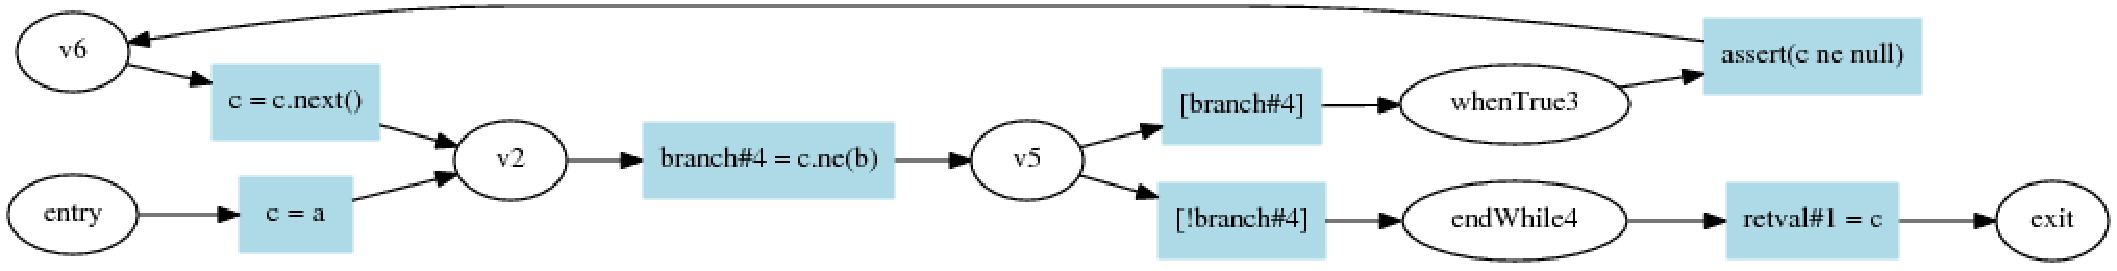
\includegraphics[scale=0.40]{images/cfg_example1}

    \caption{CFG Representation}
    \label{fig:cfg:example1}
\end{figure}

\section{Class Hierarchy}
This phase is responsible to build the complete graph representing the class
hierarchy. It is then able to provide information such as $subtypes(C) :=
\{ T ~|~ T,C \in Classes \land T \subtypeeq C \}$, which is required by later
phases.

It is worth noting that in object oriented languages such as Scala,
$subtypes()$ is generally not bounded. This is caused by the fact that most
classes are not defined as \emph{final}, so that users can extend and redefine
parts of them. Scala also defines the concept of \emph{sealed} class, forcing
all \emph{direct} subtypes to be defined in the same source file. This property
is not sufficient in our case, since it only affects direct children (children
of non-sealed parents can be defined anywhere). In other words, the
\emph{sealed} property is not transitive.

In order to provide a useful analysis, we assume whole-code analysis: we
consider that classes analyzed represent the entire program, which allows us to
have bounded $subtypes()$ sets.  We argue that it is a reasonable and pragmatic
assumption, as it wouldn't be useful to analyze classes while assuming that
most methods could be in fact completely rewritten in imaginary sub-classes.

\section{Type Analysis}

\subsection{Introduction}
Object oriented languages such as Scala implement \emph{dynamic dispatch}: the
target of a method call is only determined at runtime, based on the actual
runtime type of the receiver. This feature is essential in object oriented
languages as it allows subtype polymorphism. Consider the Scala code in
Figure~\ref{fig:ta:example1}: the declared type of \lstinline{obj} in
\lstinline{A.test} is \lstinline{A}, but the target of the method call could
either be \lstinline{A.foo} or \lstinline{B.foo}, based on the actual type of
the value of \lstinline{obj}, which is only fully determined at runtime.

\begin{figure}[h]
    \centering
\begin{minipage}[tl]{0.6\linewidth}
    \centering
\lstset{linewidth=0.6\linewidth}
\begin{lstlisting}
class A {
  def run {
    test(new B)
  }
  def test(obj: A) {
    obj.foo()
  }
  def foo() {
    println("A")
  }
}
\end{lstlisting}
\end{minipage}
\begin{minipage}[tl]{0.6\linewidth}
    \centering
\lstset{linewidth=0.6\linewidth}
\begin{lstlisting}

class B extends A {
  override def foo() {
    println("B")
  }
}
\end{lstlisting}
\end{minipage}
    \caption{Dynamic dispatch}
    \label{fig:ta:example1}
\end{figure}

In general, every redefinitions of \lstinline{foo} in all subclasses of \lstinline{A}
could be targets of this method call. We formalize this concept by associating
for each method call a set of targets, $CT$. For this example, we have:
\begin{eqnarray*}
    CT(\verb/obj.foo()/@p) = \{A.foo, B.foo\}
\end{eqnarray*}
where $p$ is the program point--or label uniquely identifying the call.

Type analysis is responsible for computing this set of targets $CT$. For this
analysis to be valid, the set of targets should include all methods that could
be called at runtime. It may however be imprecise and include methods that will
never be called at runtime.

A simplistic implementation of this analysis would be the following. Consider a
call \lstinline{rec.foo()} where the receiver \lstinline{rec} is of type
\emph{T}, all subtypes of \emph{T} where method \lstinline{foo()} is redefined:
\begin{eqnarray*}
        SimpleCT(\verb/rec.foo(..)/@p) := \{C.foo ~ &|& C \in Classes \land \\
        && C \subtypeeq type(\verb/rec/) \land \\
        && \verb/foo/ \in methods(C) \}
\end{eqnarray*}
where $methods(C)$ is the set of methods explicitly (re)defined in class $C$.
This analysis is sound,
but it will often be imprecise, as illustrated in
Figure~\ref{fig:ta:example2}. Even though the type of \lstinline{obj} is
\emph{A}, so subtypes are $\{A, B\}$, the only possible target of
\lstinline{obj.foo()} is \lstinline{A.foo}.

\begin{figure}[h]
    \centering

\begin{minipage}[tl]{0.6\linewidth}
    \centering
\lstset{linewidth=0.6\linewidth}
\begin{lstlisting}
class A {
    def invoke {
        val obj = new A()
        obj.foo()
    }
    def foo() {
        println("A")
    }
}
\end{lstlisting}
\end{minipage}
\begin{minipage}[tl]{0.6\linewidth}
    \centering
\lstset{linewidth=0.6\linewidth}
\begin{lstlisting}

class B extends A {
    override def foo() {
        println("B")
    }
}
\end{lstlisting}
\end{minipage}
    \caption{Precise call}
    \label{fig:ta:example2}
\end{figure}

A lack of precision in this analysis will only result in poorer time
performances, and will not impact the precision of the overall analysis.
Indeed, this analysis is only used to build the initial callgraph. A more
precise type analysis will be
performed during the pointer analysis phase. 

\subsection{Analysis}
Analyzing the targets of method calls can be reduced to analyzing the runtime
types of variables. Those types then fully determines the targets of the call.
Our analysis will thus analyze types that could occur at runtime, for every
variables present in the code. We distinguish three types of variables:
\begin{enumerate}
    \item \verb/A.f/: Field \verb/f/ of class \verb/A/.
    \item \verb/arg/: Argument \verb/arg/ of the function.
    \item \verb/locVar/: Local variable \verb/locVar/.
\end{enumerate}

For each of these variable occurrences in the code, our analysis will compute
the set of runtime types, that we will call \emph{ComputedTypes}, as opposed to
\emph{RuntimeTypes} which is the set of all types that could occur in runtime.
For the resulting type analysis to be valid, the set of computed object types
should be a superset of the types of values assigned to those variables at
runtime.  We thus have the following validity requirement:
\begin{eqnarray*}
    \forall v \in Variables: RuntimeTypes(v) \subseteq ComputedTypes(v)
\end{eqnarray*}

To compute the set of types at runtime, we track values assigned to those
variables. When doing this, we immediately face two non-trivial problems:
\begin{enumerate}
    \item The values of arguments are determined by call-sites, determining
    call-sites of a certain method is analogous to determining call targets,
    which is the purpose of type analysis.

    \item Fields can be assigned from multiple locations, within various
    methods. Again, determining whether those methods are
    called, and in which order, require type analysis.
\end{enumerate}

Both of those problems could be solved using a fix-point mechanism. However, at
the cost of some precision, we decided to fall back to a simple implementation
for both arguments and fields:
\begin{eqnarray*}
    ComputedTypes(\verb/A.f/) &:=& \{ T ~|~ T \subtypeeq type(\verb/A.f/) \} \\
    ComputedTypes(\verb/arg/) &:=& \{ T ~|~ T \subtypeeq type(\verb/arg/) \} \\
\end{eqnarray*}
where $type()$ is the type inferred by the compiler.

For local variables, we run a flow-sensitive, context-insensitive, abstract
interpretation-based analysis. This analysis computes, at every program point,
the set of all types assigned to local variables. For this analysis to be
efficient, we split the type information into two sets $T_{sub}$ and $T_{ex}$.
$T_{ex}$ contains "exact" types, while $T_{sub}$ contains types from which we
need to also consider subtypes. This split is useful for two reasons: first, it
allows us to keep a small representation for subtypes of, e.g. Object. Second,
it lets us delay the resolution of the actual types until the last moment.
Globally, storing runtime types with that representation is much more memory
efficient than storing a plain set of potential types. We formally define the
type information as follows:
\begin{eqnarray*}
    TypeInfo &:=& \langle T_{sub} \subtypeeq Types, T_{ex} \subtypeeq Types\rangle \\
    Types    &:=& Classes \cup \{ Array[T] ~|~ T \in Types \} \\
\end{eqnarray*}


We thus have a point-wise lattice \emph{L} over pairs of sets of types. Its
point-wise lowest upper bound operation is naturally defined as:
$$
    \langle T_{sub_a}, T_{ex_a} \rangle \sqcup  \langle T_{sub_b}, T_{ex_b} \rangle =  \langle T_{sub_a} \cup T_{sub_b}, T_{ex_a} \cup T_{ex_b} \rangle
$$
We outline in Figure~\ref{fig:ta:tf}
the abstraction function for important values.
\FloatBarrier
\begin{figure}[h]
    \centering

    \begin{tabular}{ l | l }
        Expression $ex$       & Abstract Value $\alpha(ex)$\\
        \hline
        \verb/new A/          & $\langle \emptyset, \{ A \} \rangle$ \\
        \verb/null/           & $\langle \emptyset, \emptyset \rangle$ \\
        \verb/A.f/            & $\langle\{type(\verb/A.f/)\}, \{type(\verb/A.f/)\} \rangle$ \\
        \verb/rec.meth(..)/   & $\langle\{type(\verb/rec.meth/)\}, \{type(\verb/rec.meth/)\} \rangle$ \\
    \end{tabular}

    \caption{Abstraction function $\alpha$, where $type()$ returns the declared
    type.}
    \label{fig:ta:tf}
\end{figure}

The number of used types, although infinite in theory, is finite for a given
program given that it typechecks. For this reason, we can argue that this
analysis terminates, since there are only finite ascending chains in the
lattice as $\mathcal{T}(Types)$ is finite. We also have a trivially monotonic
transfer function.

When the fix-point is reached, we can derive the set of call targets \emph{CT}
for each method call using $facts$ computed at their program point:
\begin{eqnarray*}
    CT(\verb/rec.meth(..)/ @ p) := \{ T.meth ~|~ T \in \gamma(facts@p(\verb/rec/)) \land \verb/meth/ \in methods(T) \}
\end{eqnarray*}
where $\gamma$ is the concretisation function, computing the entire set of
types that the pair represents:

$$
\gamma(\langle T_{sub}, T_{ex} \rangle ) := \{ T ~|~ \exists S \in T_{sub}. T \subtype S\} \cup T_{ex}
$$

This analysis provides us with a relatively precise information on call
targets. We believe that the obvious lack of precision in the presence of
fields and arguments is not problematic, since the callgraph is only used to
determine groups of mutually recursive functions. For this reason, this
analysis is arguably overly precise. However, we have seen that it is
sufficiently fast in practice.


\end{document}
